%%%%%%%%%%%%%%%%%%%%%%%%%%%%%%%%%%%%%%%%%%%%%%%%%%%%%%%%%%%%%%%%%%%%%%
\begin{frame}[fragile]\frametitle{}
\begin{center}
{\Large Recursion}
\end{center}

\end{frame}

%%%%%%%%%%%%%%%%%%%%%%%%%%%%%%%%%%%%%%%%%%%%%%%%%%%%%%%%%%%%%%%%%%%%%%
\begin{frame}[fragile]
	\frametitle{What is Recursion?}
		\begin{itemize}
			\item Function calling itself with a subproblem.
			\item Possible where: performing same operations multiple times with different/smaller inputs
			\item Smallest condition is base/breaking and simplest. Else, infinite loop will occur.
		\end{itemize}
		
		\begin{lstlisting}
		def foo(input):
			if input == 1:
				return "Got solution"
			else:
				foo(input - 1)
		\end{lstlisting}
\end{frame}

%%%%%%%%%%%%%%%%%%%%%%%%%%%%%%%%%%%%%%%%%%%%%%%%%%%%%%%%%%%%%%%%%%%%%%
\begin{frame}[fragile]
	\frametitle{Why Recursion?}
		\begin{itemize}
			\item Recursive thinking helps bring out cleaner/understandable solution.
			\item Subproblem has to be similar to the original one.
			\item Can be converted into iterative solution
			\item Heavily used in Trees and Graphs data structures.
		\end{itemize}
\end{frame}

%%%%%%%%%%%%%%%%%%%%%%%%%%%%%%%%%%%%%%%%%%%%%%%%%%%%%%%%%%%%%%%%%%%%%%
\begin{frame}[fragile]
	\frametitle{How Recursion works?}
		\begin{itemize}
			\item Need to store callee method pointer somewhere so as to come back once the function execution is over.
			\item Methods are pushed in to call-stack and pop-ed once execution is over.
		\end{itemize}
		
\begin{center}
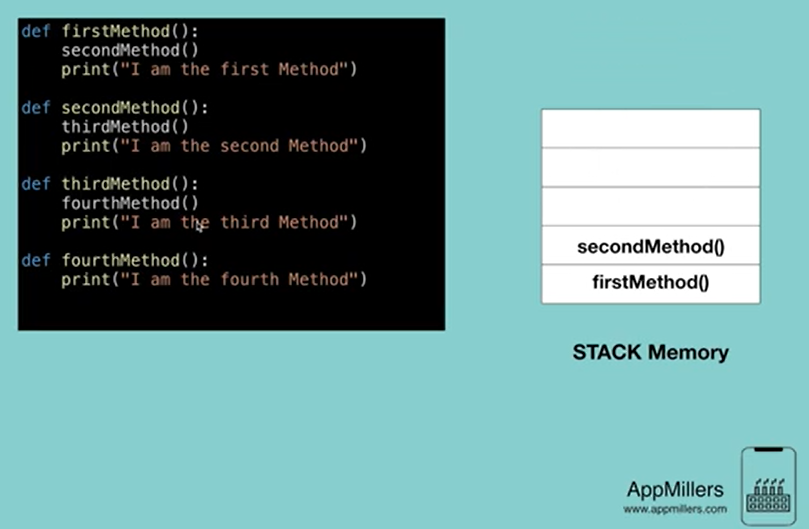
\includegraphics[width=0.75\linewidth,keepaspectratio]{recursive1.png}
\end{center}


\end{frame}

%%%%%%%%%%%%%%%%%%%%%%%%%%%%%%%%%%%%%%%%%%%%%%%%%%%%%%%%%%%%%%%%%%%%%%
\begin{frame}[fragile]
	\frametitle{How Recursion works?}

In recursion, all these methods are same, but with smaller arguments.
		
		
\begin{center}
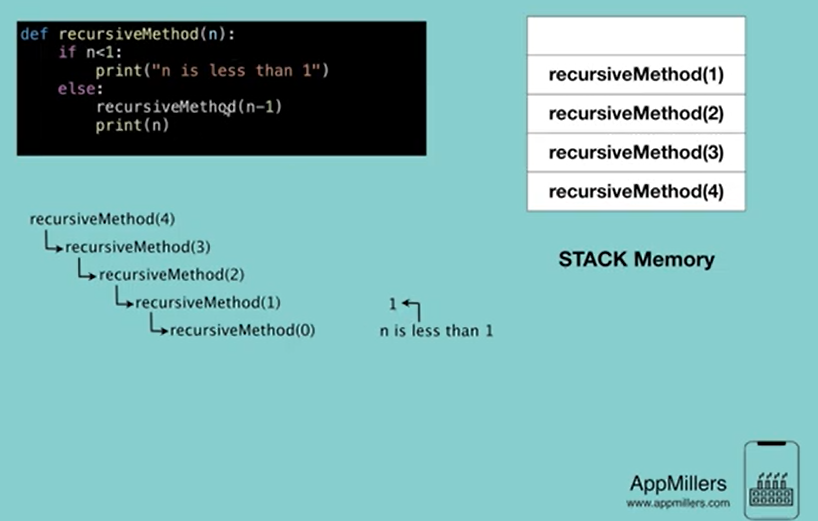
\includegraphics[width=\linewidth,keepaspectratio]{recursive3.png}
\end{center}


\end{frame}


%%%%%%%%%%%%%%%%%%%%%%%%%%%%%%%%%%%%%%%%%%%%%%%%%%%%%%%%%%%%%%%%%%%%%%
\begin{frame}[fragile]
	\frametitle{Write in 3 Steps}
		\begin{itemize}
			\item Identify recursive portion
			$n! = n * (n-1)!$
			
			\begin{lstlisting}
			def factorial(n):
				return n * factorial(n-1)
			\end{lstlisting}
			
			\item 

			\item Identify breaking condition to stop infinite loop
			$1! = 1; 0! = 1$
			
			\begin{lstlisting}
			def factorial(n):
			if n in [0,1]:
				return 1
			else:
				return n * factorial(n-1)
			\end{lstlisting}	
			
			\item 

			\item Identify constraints, unconditional case.
			$n > 0$
			
			\begin{lstlisting}
			def factorial(n):
			assert n >= 0 and int(n) == n, "number must be positive integer"
			if n in [0,1]:
				return 1
			else:
				return n * factorial(n-1)
			\end{lstlisting}
			
		\end{itemize}
\end{frame}

%%%%%%%%%%%%%%%%%%%%%%%%%%%%%%%%%%%%%%%%%%%%%%%%%%%%%%%%%%%%%%%%%%%%%%
\begin{frame}[fragile]
	\frametitle{Example: Fibonacci Numbers}


\begin{center}
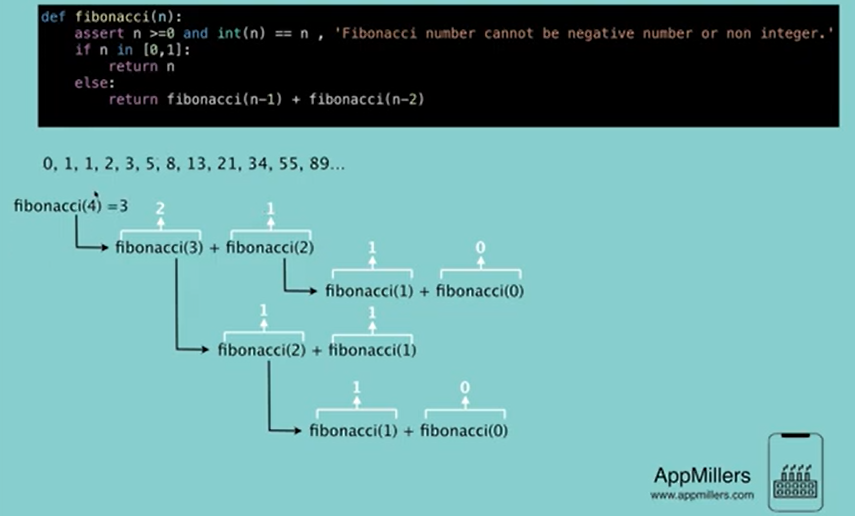
\includegraphics[width=\linewidth,keepaspectratio]{recursive4.png}
\end{center}


\end{frame}

%%%%%%%%%%%%%%%%%%%%%%%%%%%%%%%%%%%%%%%%%%%%%%%%%%%%%%%%%%%%%%%%%%%%%%
\begin{frame}[fragile]
	\frametitle{Example: Sum of Digits}

Digits of a number are isolated using powers of 10 and taking remainder out.

$f(n) = n\%10 + f(n/10)$

\begin{lstlisting}
def sumofDigits(n):
    assert n>=0 and int(n) == n , 'The number has to be a postive integer only!'
    if n == 0:
        return 0
    else:
        return int(n%10) + sumofDigits(int(n/10))
\end{lstlisting}


\end{frame}

%%%%%%%%%%%%%%%%%%%%%%%%%%%%%%%%%%%%%%%%%%%%%%%%%%%%%%%%%%%%%%%%%%%%%%
\begin{frame}[fragile]
	\frametitle{Exercise: Power of a Number}

Hint: $x^n = x * x^{n-1}$



\end{frame}

%%%%%%%%%%%%%%%%%%%%%%%%%%%%%%%%%%%%%%%%%%%%%%%%%%%%%%%%%%%%%%%%%%%%%%
\begin{frame}[fragile]
	\frametitle{Solution: Power of a Number}

\begin{lstlisting}
def power(base,exp):
    if exp == 0:
        return 1
    if(exp==1):
        return(base)
    if(exp!=1):
        return (base*power(base,exp-1))
\end{lstlisting}


\end{frame}

%%%%%%%%%%%%%%%%%%%%%%%%%%%%%%%%%%%%%%%%%%%%%%%%%%%%%%%%%%%%%%%%%%%%%%
\begin{frame}[fragile]
	\frametitle{Exercise: Greatest Common Divisor}
		\begin{itemize}
			\item Greatest Common Divisor: highest factor of two numbers. 
			\item Take one instance of duplicate factors. E.g. $gcd(8,12); 8 = 2 x 2 x 2; 12 = 2 x 2 x 3; gcd(8,12) = 4$. 
			\item Euclidean algorithm: Divide bigger with smaller, then reminder with smaller, till reminder is 0.
				\begin{itemize}
					\item $gcd(48,18)$. 
					\item Step 1: $48/18 = 2$ remainder 12
					\item Step 2: $18/12 = 1$ remainder 6
					\item Step 3: $12/6 = 2$ remainder 0
					\item Answer = 6
				\end{itemize}			
			\item Hint: $ gcd(a,0) = a; gcd(a,b) = gcd(b, a mod b)$
		\end{itemize}
\end{frame}

%%%%%%%%%%%%%%%%%%%%%%%%%%%%%%%%%%%%%%%%%%%%%%%%%%%%%%%%%%%%%%%%%%%%%%
\begin{frame}[fragile]
	\frametitle{Solution: Greatest Common Divisor}

		\begin{lstlisting}
def gcd(a, b):
    assert int(a) == a and int(b) == b, 'The numbers must be integer only!'
    if a < 0:
        a = -1 * a
    if b < 0:
        b = -1 * b
    if b == 0:
        return a
    else:
        return gcd(b, a%b)		
		\end{lstlisting}
		
\end{frame}


%%%%%%%%%%%%%%%%%%%%%%%%%%%%%%%%%%%%%%%%%%%%%%%%%%%%%%%%%%%%%%%%%%%%%%
\begin{frame}[fragile]
	\frametitle{Example: Reverse a String}

		\begin{lstlisting}
def reverse(strng):
    if len(strng) <= 1:
      return strng
    return strng[len(strng)-1] + reverse(strng[0:len(strng)-1])


print(reverse('python')) # 'nohtyp'
print(reverse('appmillers')) # 'srellimppa'
		\end{lstlisting}
		
\end{frame}

%%%%%%%%%%%%%%%%%%%%%%%%%%%%%%%%%%%%%%%%%%%%%%%%%%%%%%%%%%%%%%%%%%%%%%
\begin{frame}[fragile]
	\frametitle{Example: Is Palindrome}

		\begin{lstlisting}
def isPalindrome(strng):
    if len(strng) == 0:
        return True
    if strng[0] != strng[len(strng)-1]:
        return False
    return isPalindrome(strng[1:-1])

print(isPalindrome('awesome')) # false
print(isPalindrome('foobar')) # false
print(isPalindrome('tacocat')) # true
print(isPalindrome('amanaplanacanalpanama')) # true
print(isPalindrome('amanaplanacanalpandemonium')) # false
		\end{lstlisting}
		
\end{frame}


%%%%%%%%%%%%%%%%%%%%%%%%%%%%%%%%%%%%%%%%%%%%%%%%%%%%%%%%%%%%%%%%%%%%%%
\begin{frame}[fragile]
	\frametitle{Recursive vs Iterative}

Converting recursive function to iterative function is difficult many a times.

\begin{center}
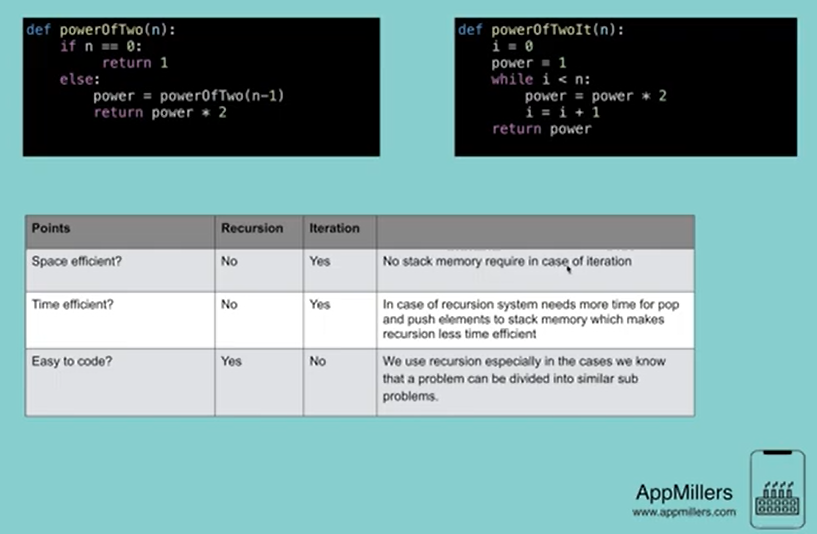
\includegraphics[width=\linewidth,keepaspectratio]{recursive2.png}
\end{center}


\end{frame}

%%%%%%%%%%%%%%%%%%%%%%%%%%%%%%%%%%%%%%%%%%%%%%%%%%%%%%%%%%%%%%%%%%%%%%
\begin{frame}[fragile]
	\frametitle{Pros and Cons}
		\begin{itemize}
			\item use when its natural to divide the problem in to similar subproblems.
			\item Has extra overhead of space (stack) and time (calls)
			\item Writing can be easy but debugging is not.
			\item More natural for Trees.
		\end{itemize}
\end{frame}

